In the case of Apomorphine, it has been shown that neuroleptic drugs like Haloperidol, causing high incidences of unwanted extrapyramidal side effects(drug-induced movement disorders), suppress the Apomorphine-induced compulsive stressing, while atypical neuroleptic drugs like Clozapine, causing low incidences of extrapyramidal side effects, suppress the Apomorphine-induced motility\cite{ref13}.
\bibitem{ref13} 
Ljungberg T., Ungerstedt U. Classification of neuroleptic drugs according to their ability to inhibit apomorphine-induced locomotion and gnawing: Evidence for two different mechanisms of action. \textit{Psychopharmacology (Berl)} \textbf{56} 239-247 (1978). 





\\Unwanted side effects of neurological disorders' medications also include direct seizure induction or enhancement of seizure triggers(proconvulsant effects). \\Proconvulsant and anticonvulsant chemical compounds can be identified in the drug discovery process, by administration along with a known convulsant agent, for example, pentylenetetrazol (PTZ). PTZ administration in zebrafish will induce epileptic-like seizures, comparable to humans, with a distinct series of changes in locomotor patterns\cite{ref14}.




\\Information contained in the descriptive statistics was  visualised as a circular cladogram, having experimental groups as leaves, which were color-coded appropriately. Cladograms were  visualised for all three disease induced conditions, using two sets of descriptive statistics, differing in whether the descriptive statistics, derived from turn and turn transition, were obtained per bout length stratum. Example of a circular cladogram for the healthy and convulsant condition in Figure 5, constructed based on a set of descriptive statistics, where the turn and turn transition descriptive statistics were not obtained per bout length stratum. All circular cladograms, constructed based on Euclidean distances between the descriptive statistiscs, in Appendix B.4. 
\begin{figure}[h!]
\begin{center}
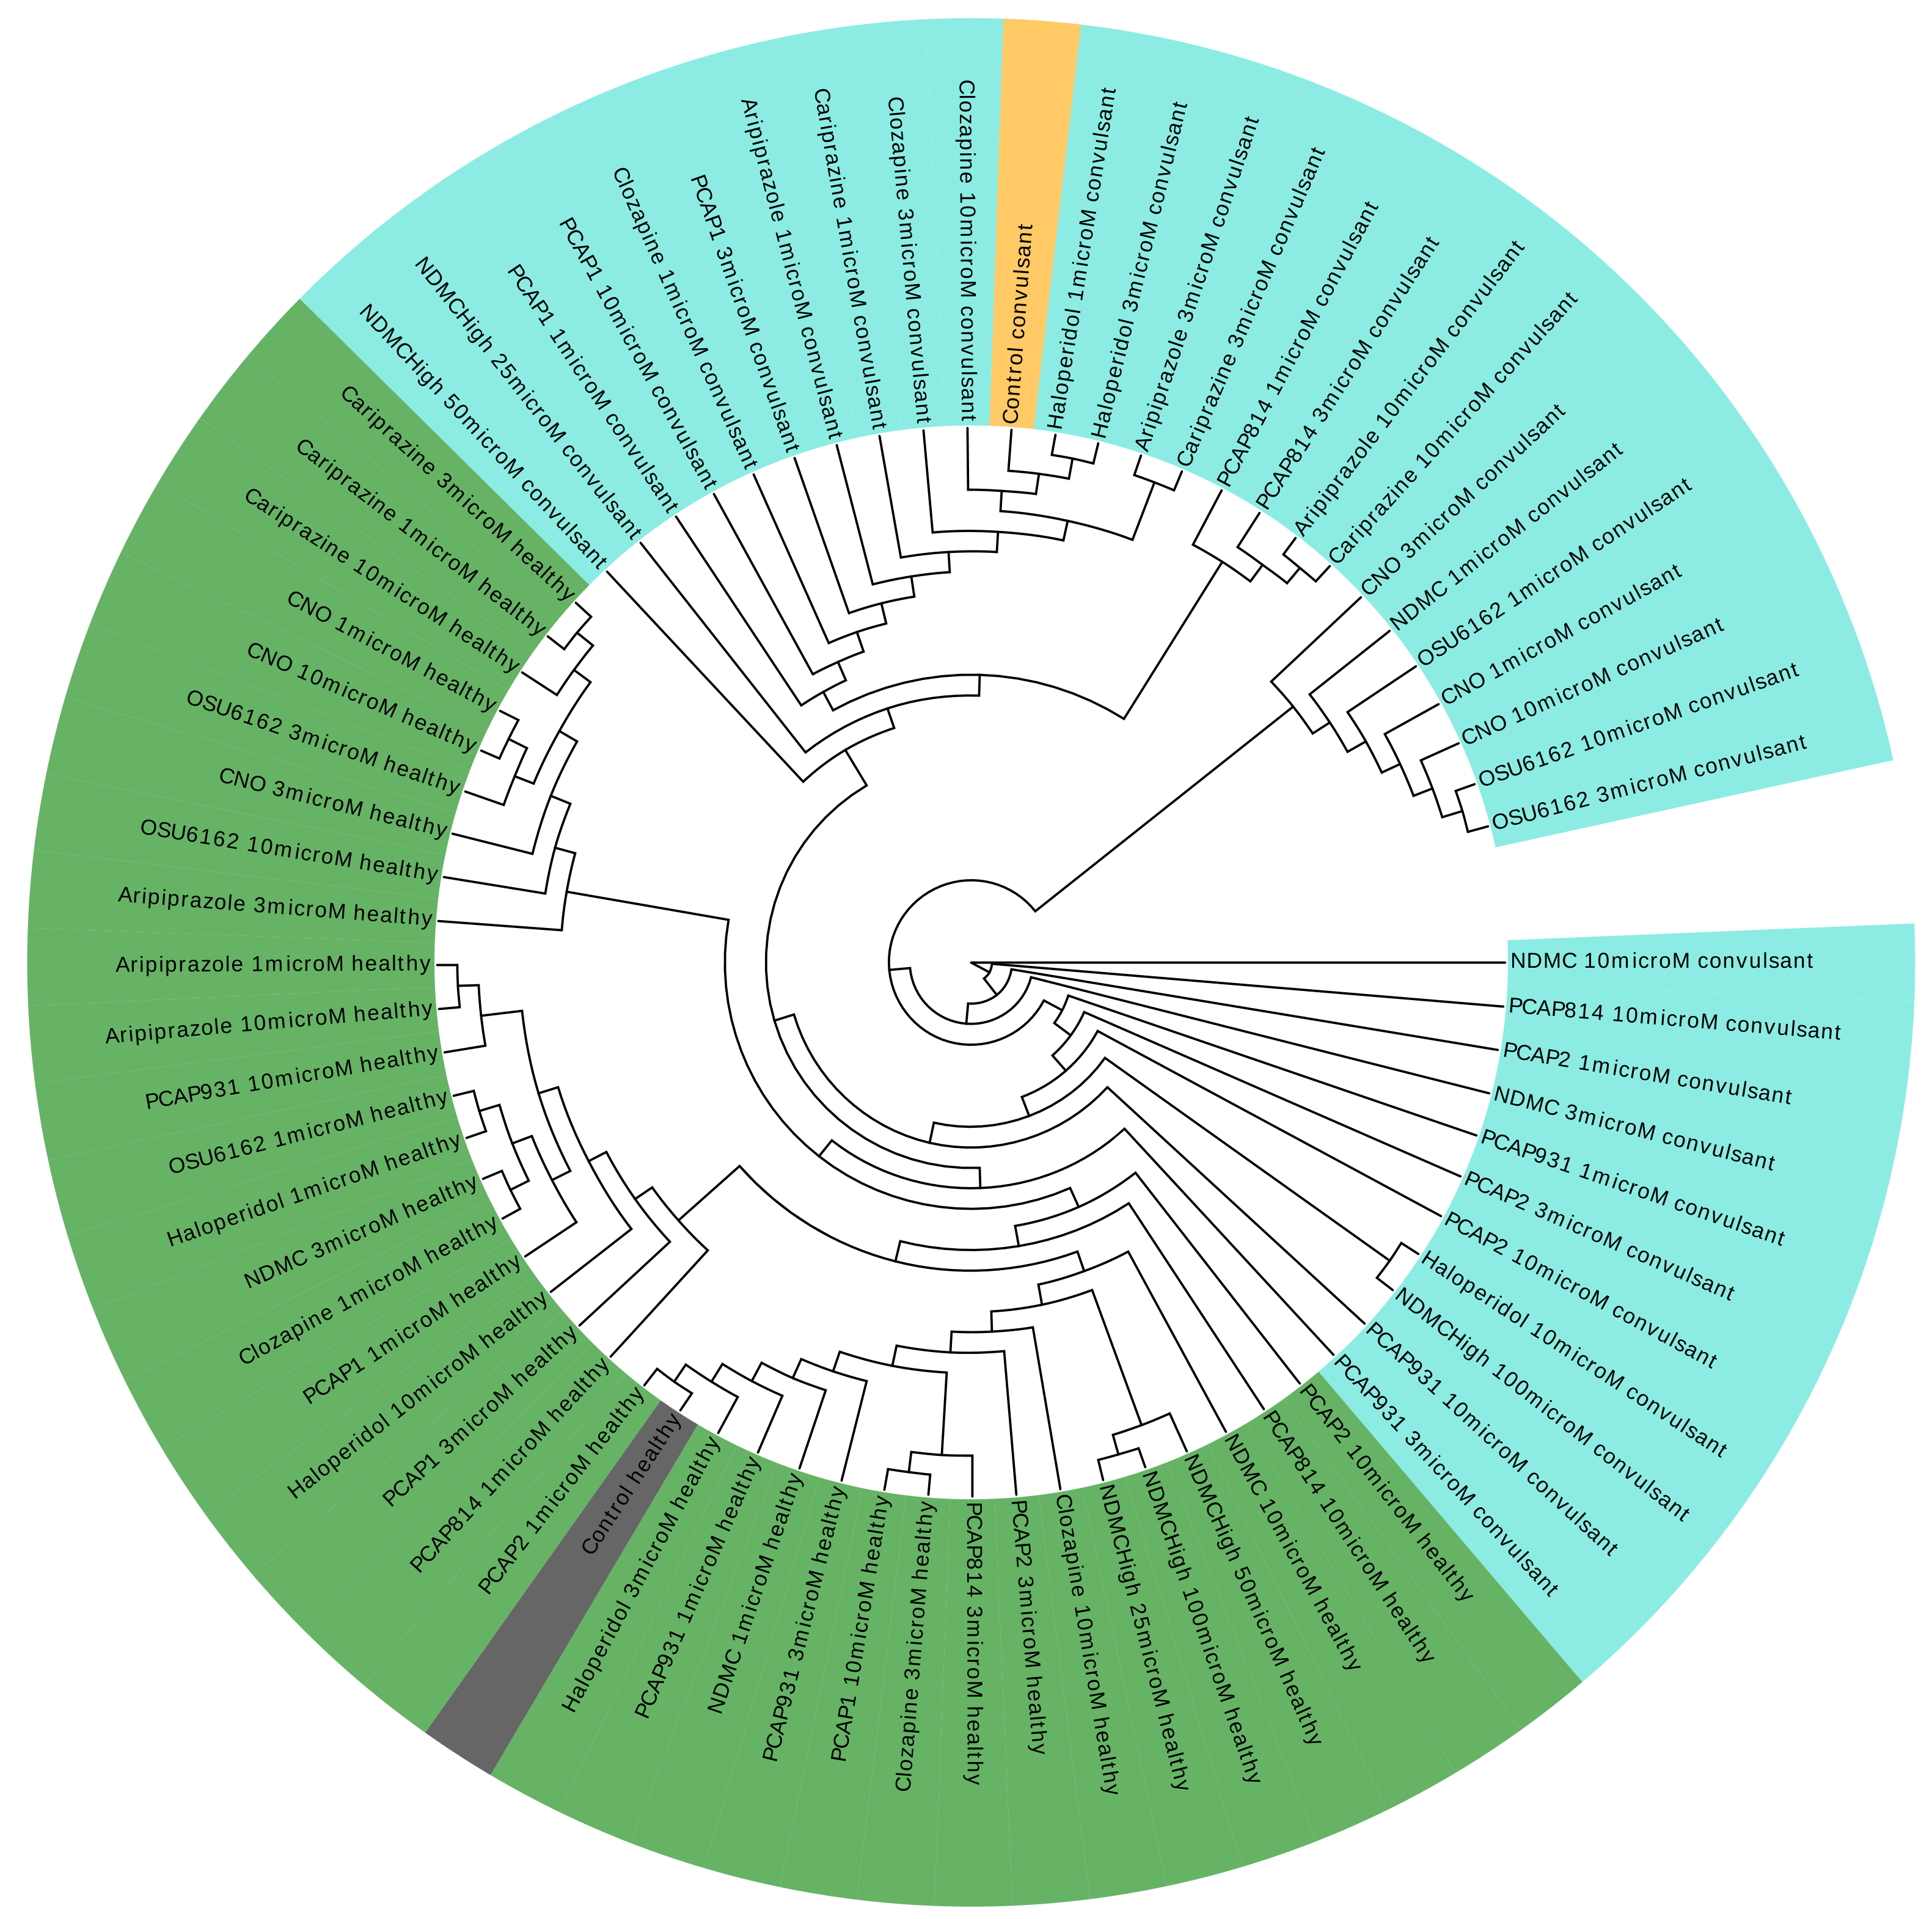
\includegraphics[width=10cm,height=10cm]{DarkPTZB2.png}
\caption{Circular cladogram, representing Euclidean distances between the descriptive statistics of all experimental groups in the healthy and convulsant condition, where the turn and turn transition descriptive statistics were not obtained per bout length stratum.}
\end{center}
\end{figure}








\subsection{Circular cladograms, based on Euclidean distances between descriptive statistics}

\begin{figure}[h!]
\begin{center}
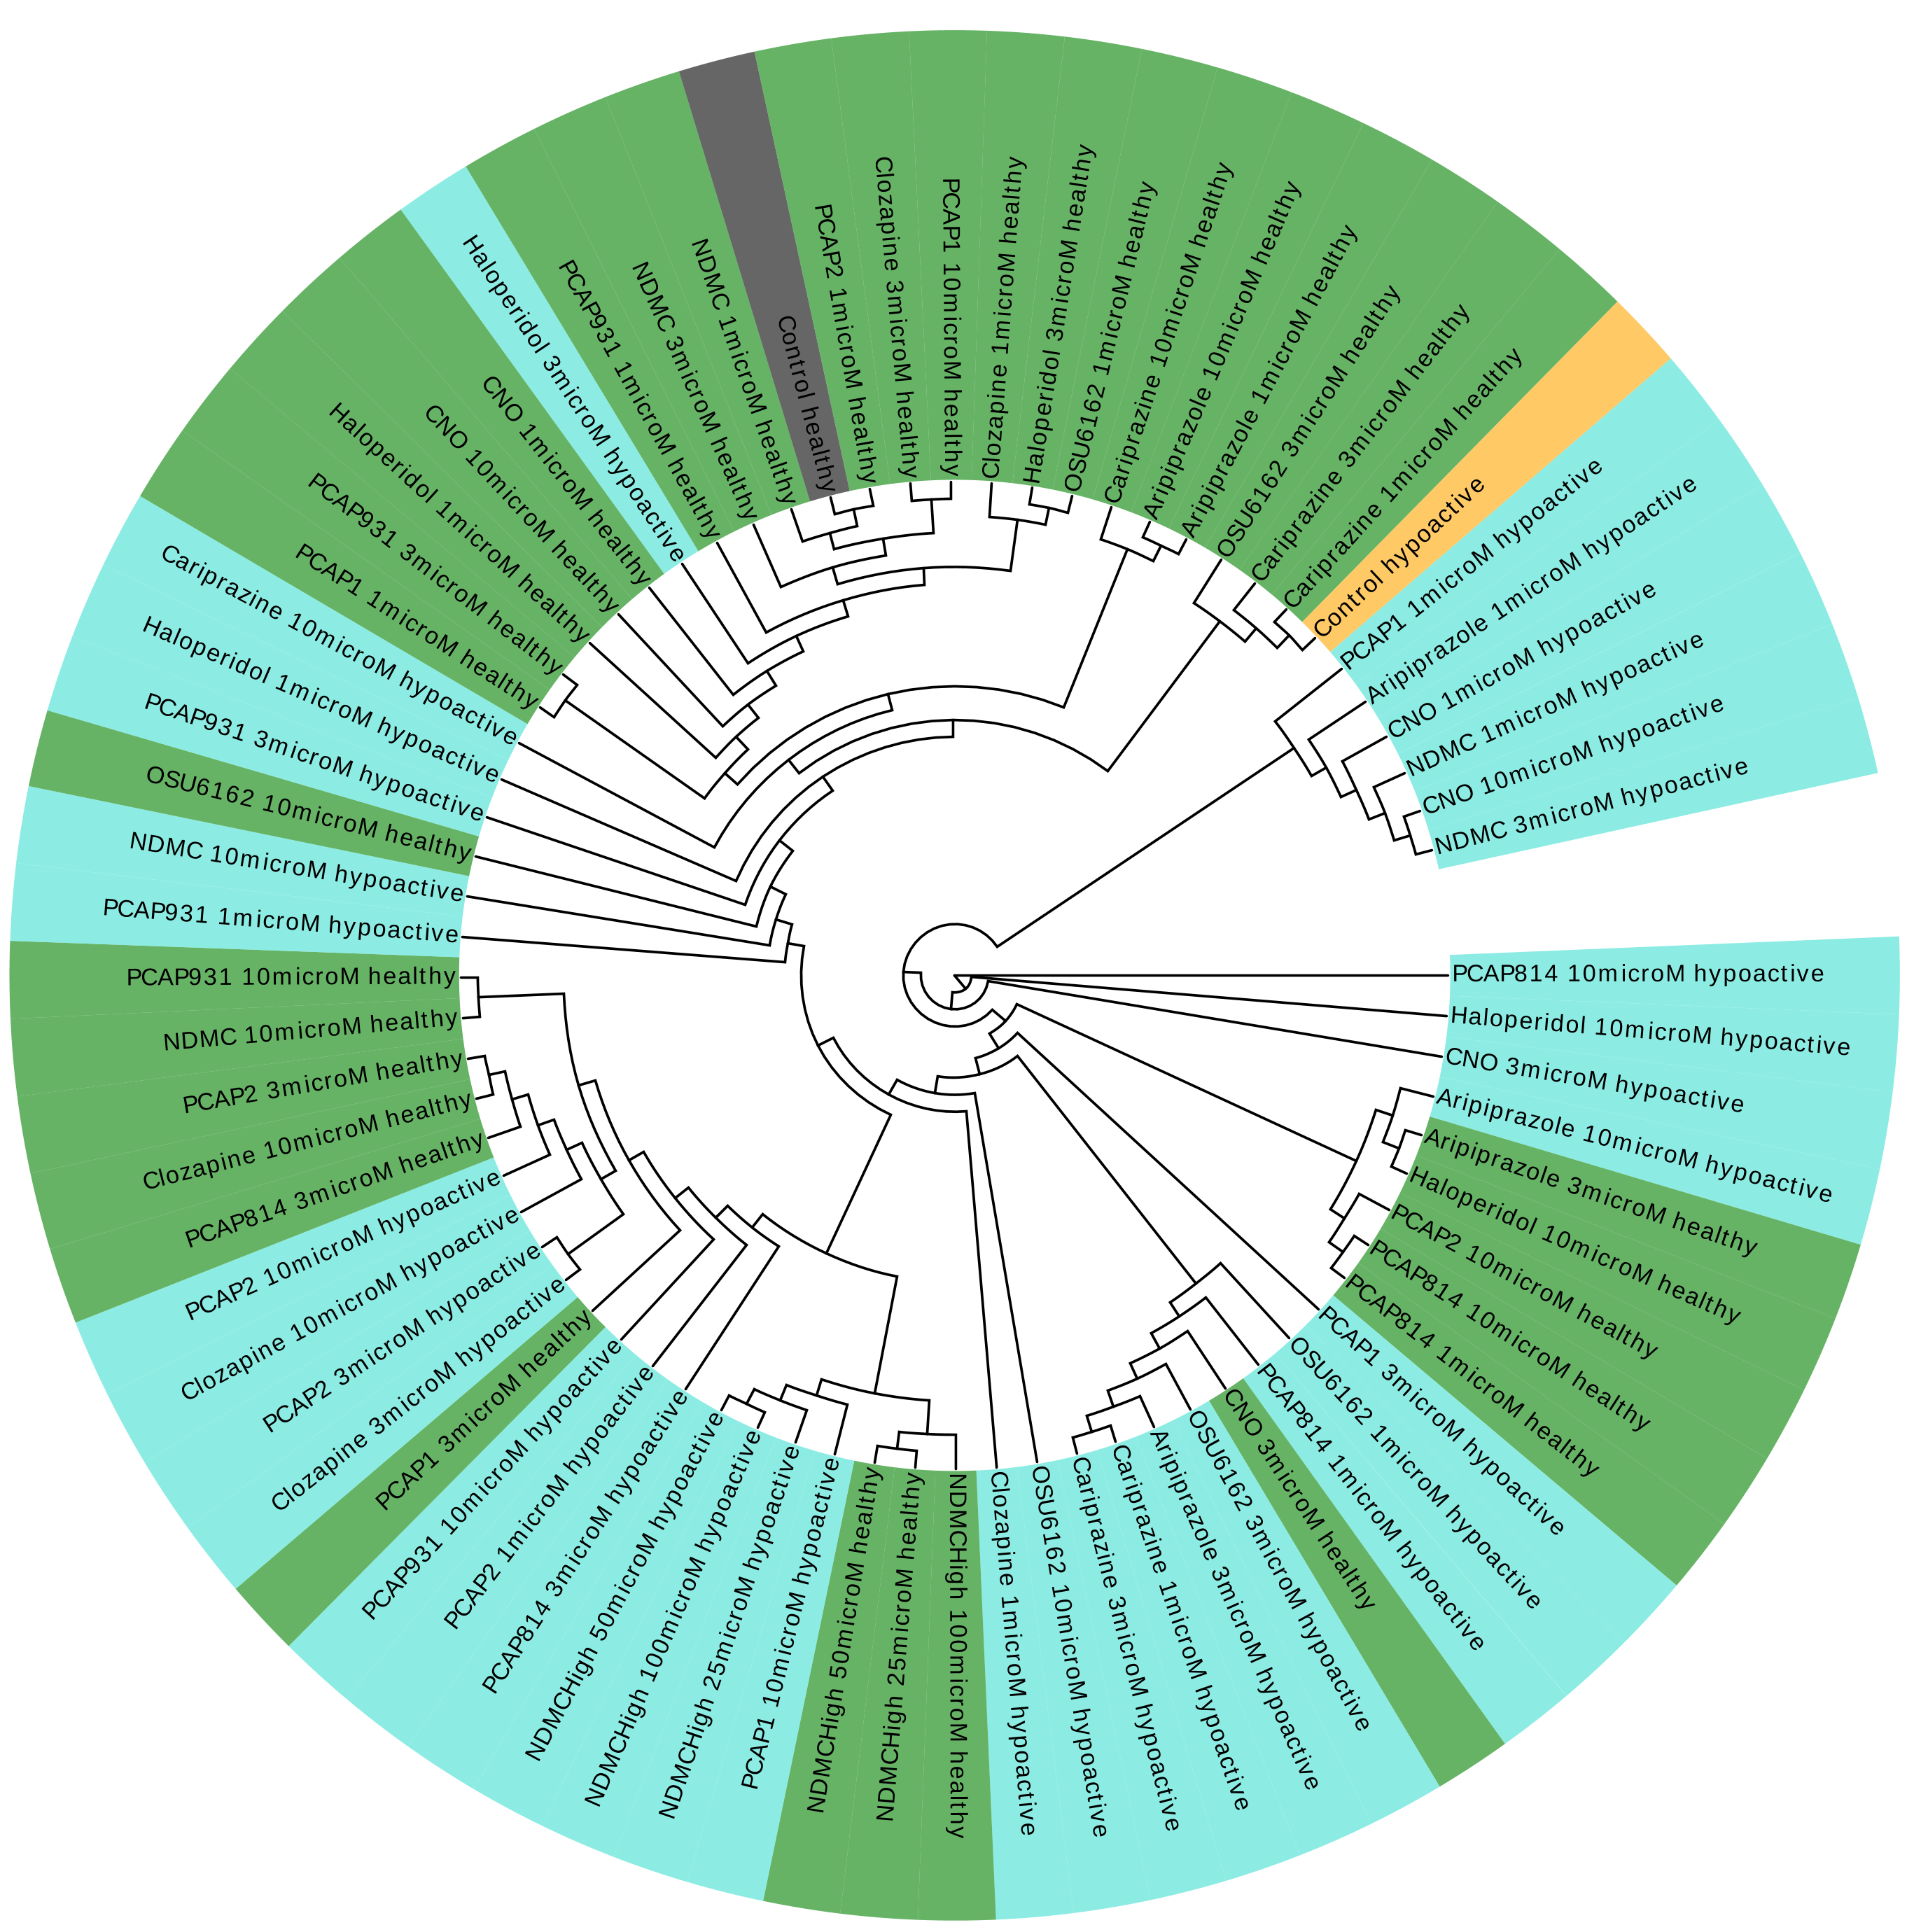
\includegraphics[width=8cm,height=7.5cm]{DarkApoLowB2.png}
\caption{Circular cladogram, representing Euclidean distances between the descriptive statistics of all experimental groups in the healthy and hypoactive condition, where the turn and turn transition descriptive statistics were not obtained per bout length stratum.}
\end{center}
\end{figure}
\begin{figure}[h!]
\begin{center}
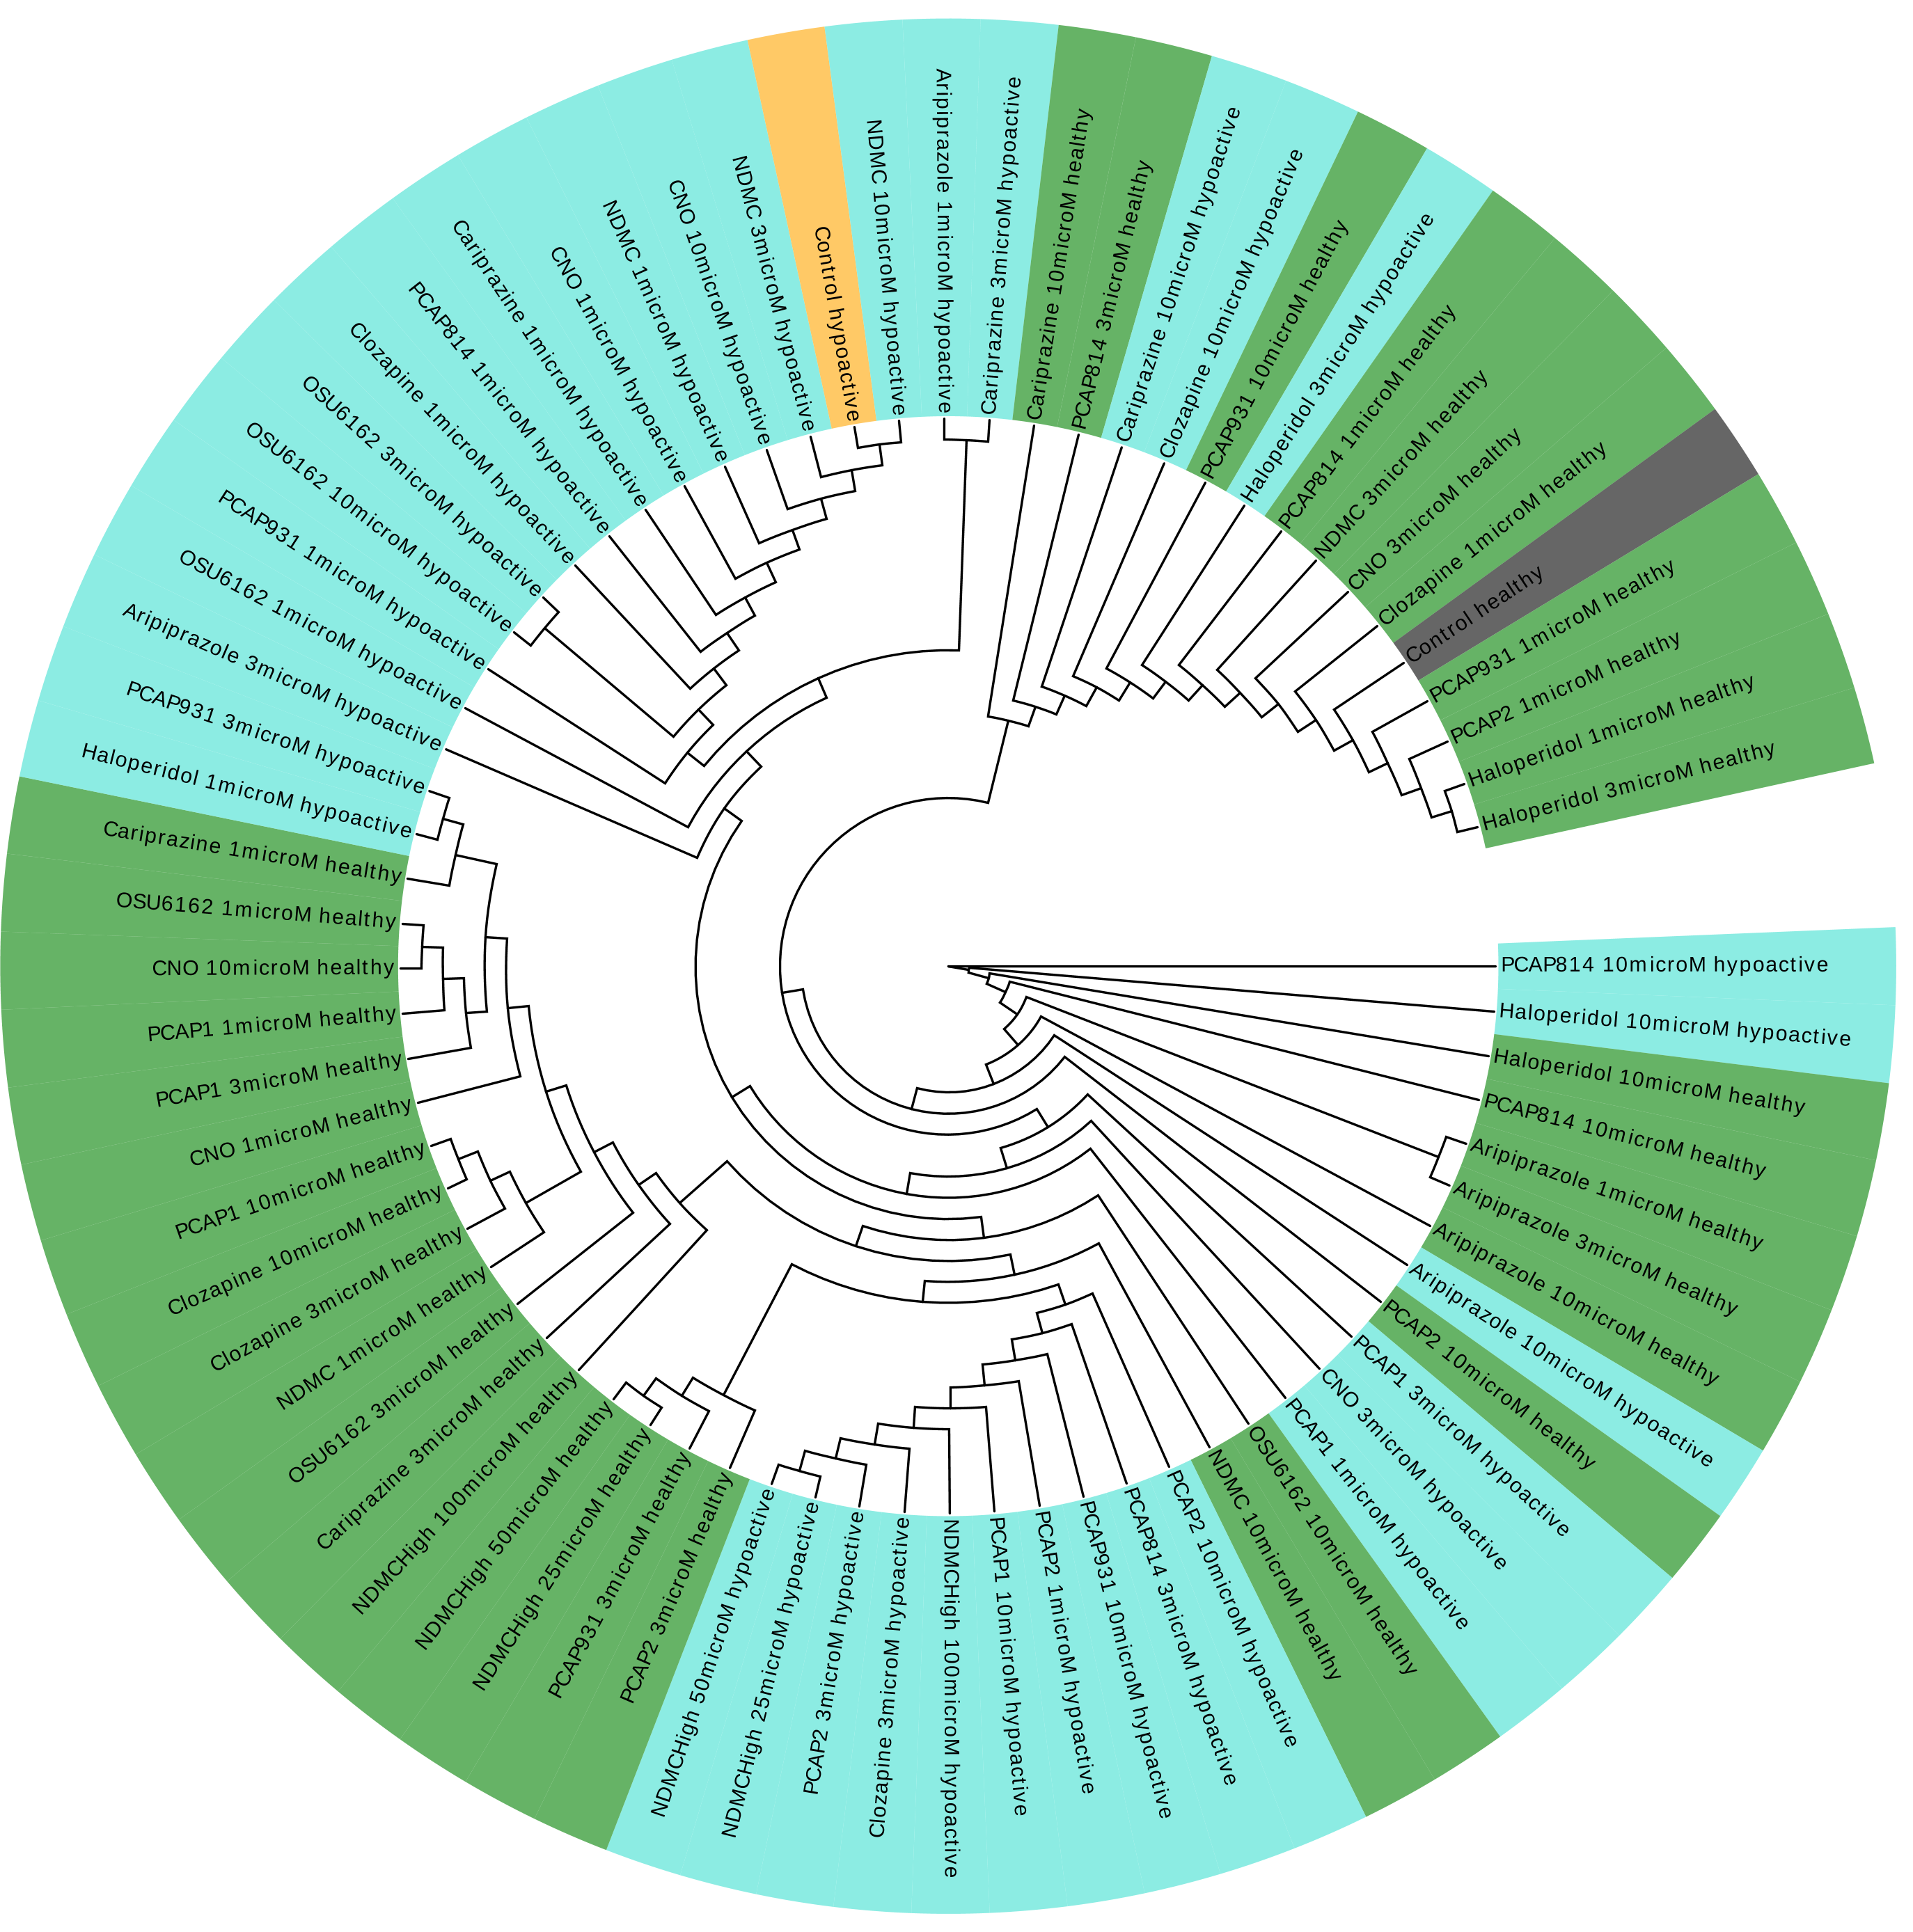
\includegraphics[width=8cm,height=7.5cm]{DarkApoLowB1.png}
\caption{Circular cladogram, representing Euclidean distances between the descriptive statistics of all experimental groups in the healthy and hypoactive condition, where the turn and turn transition descriptive statistics were obtained per bout length stratum.}
\end{center}
\end{figure}
\newpage
\begin{figure}[h!]
\begin{center}
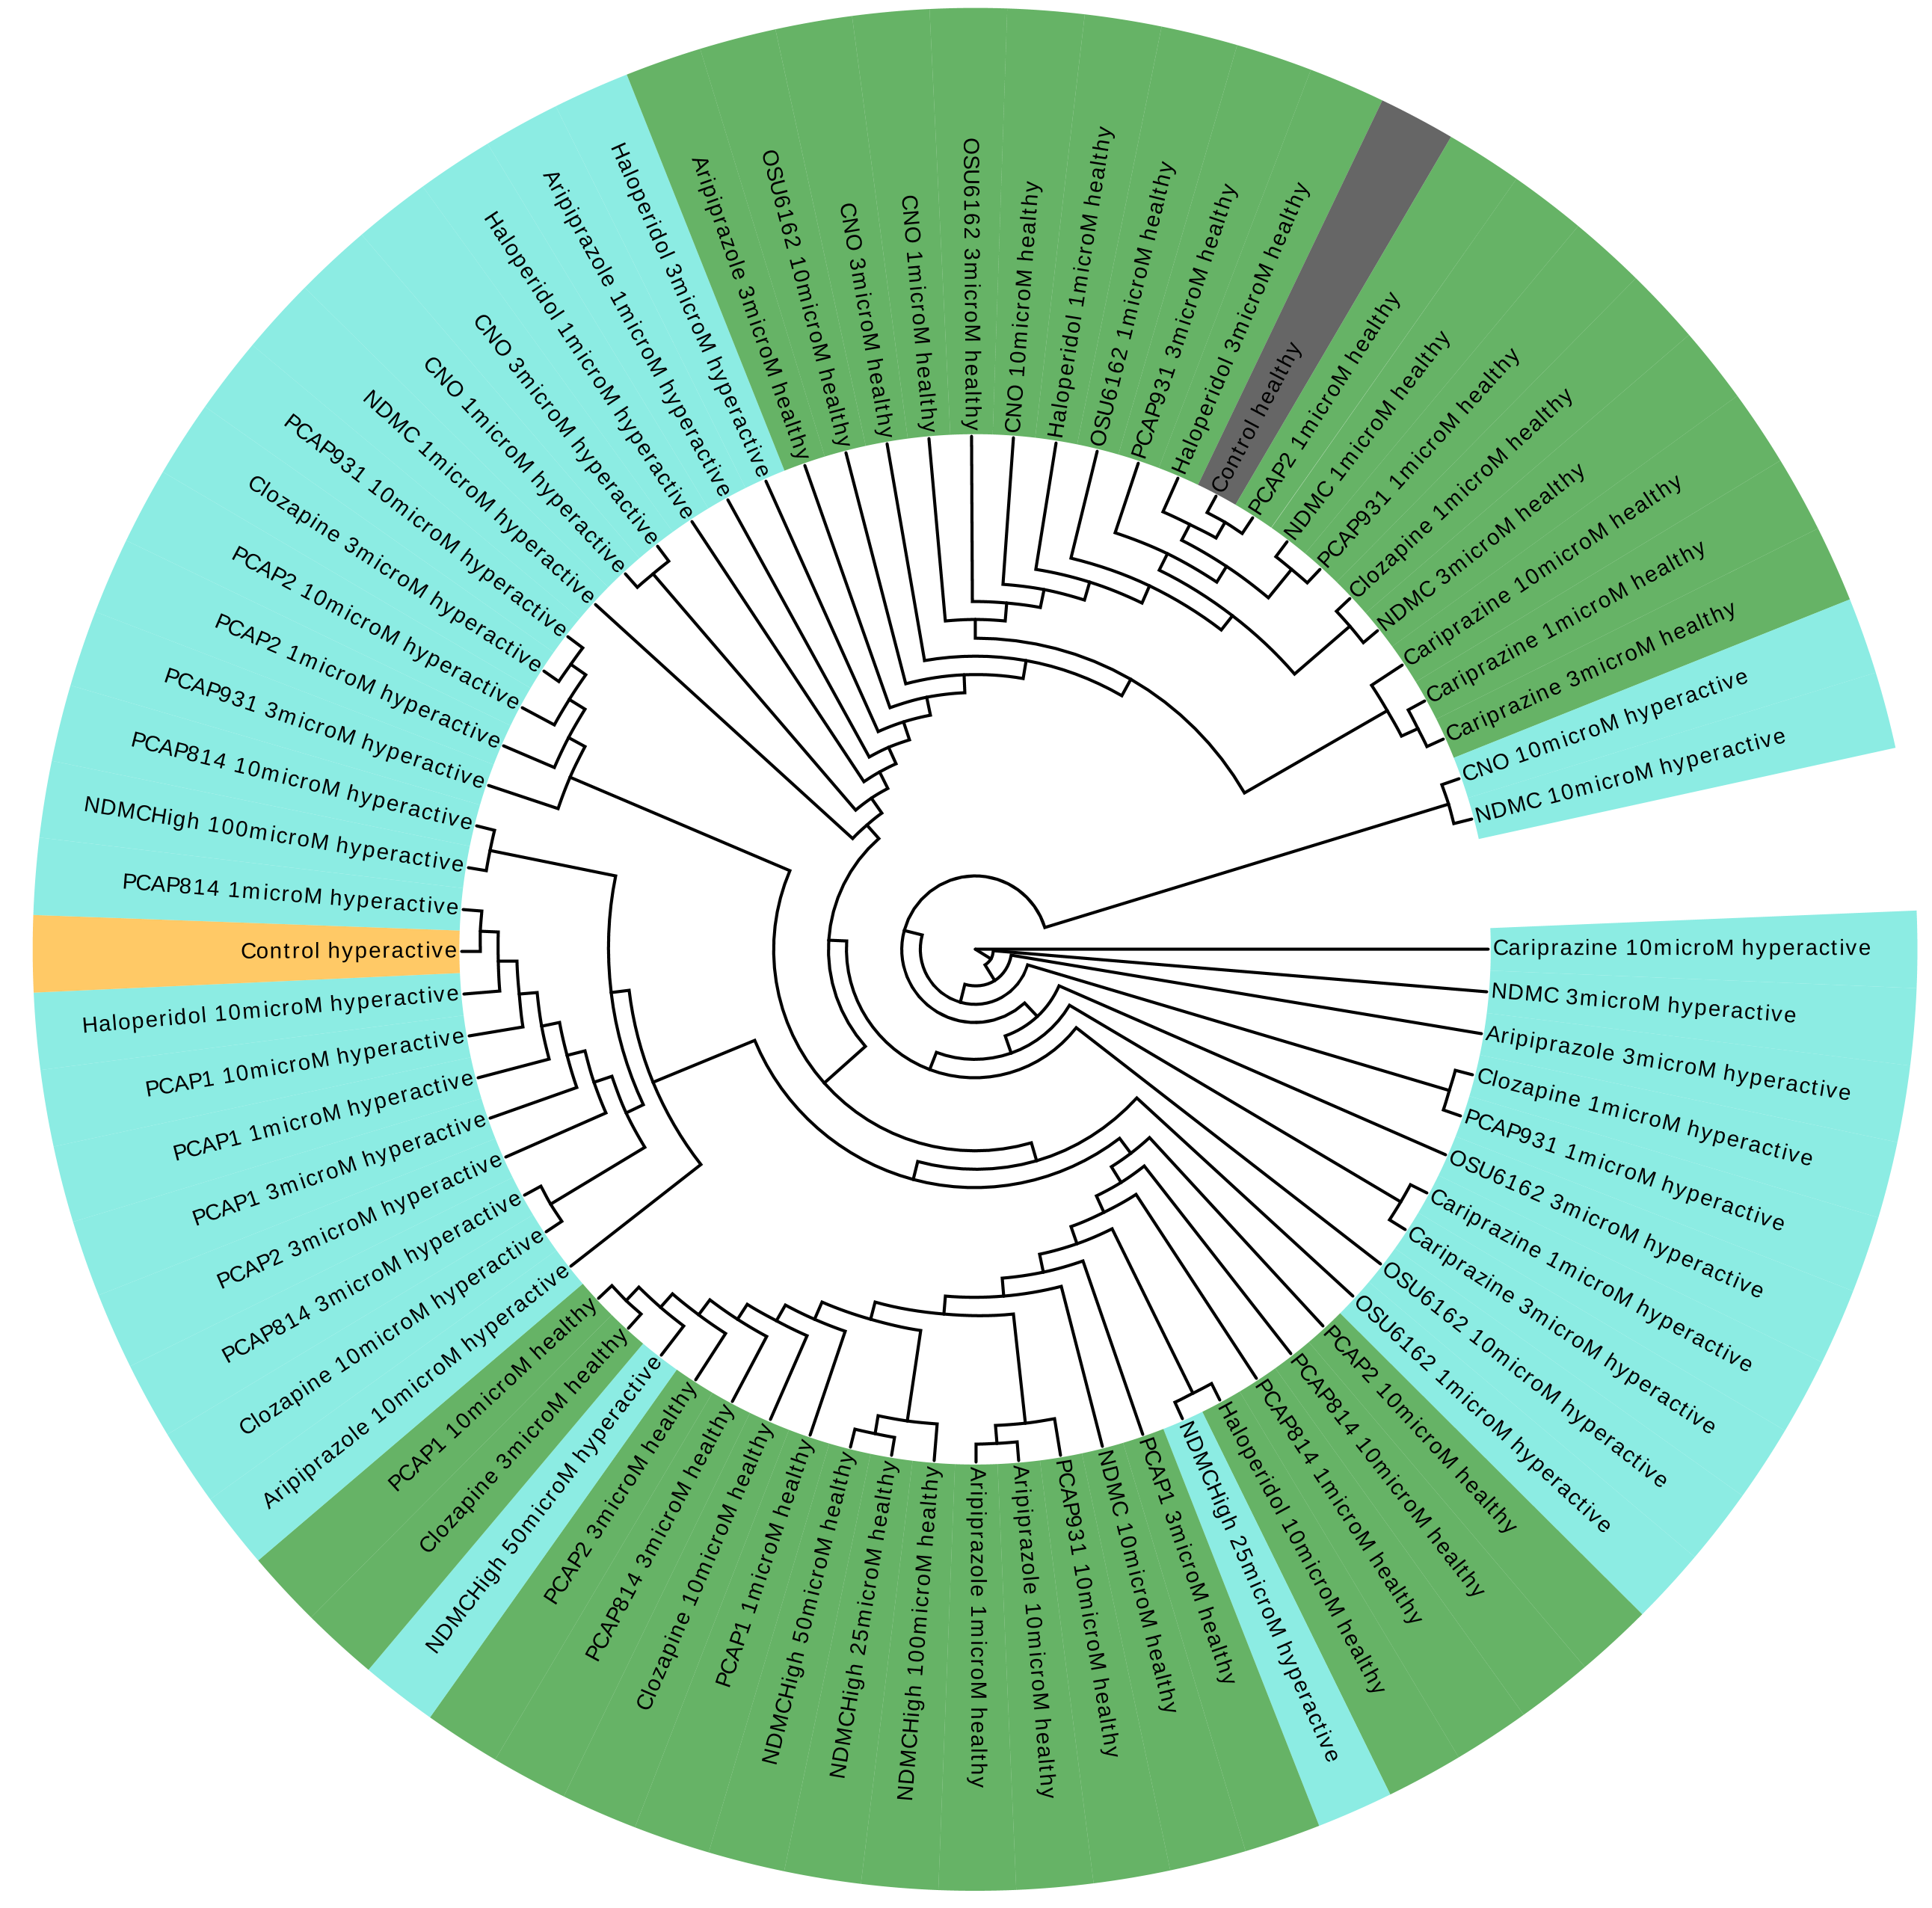
\includegraphics[width=8cm,height=8cm]{DarkApoHighB2.png}
\caption{Circular cladogram, representing Euclidean distances between the descriptive statistics of all experimental groups in the healthy and hyperactive condition, where the turn and turn transition descriptive statistics were not obtained per bout length stratum.}
\end{center}
\end{figure}
\begin{figure}[h!]
\begin{center}
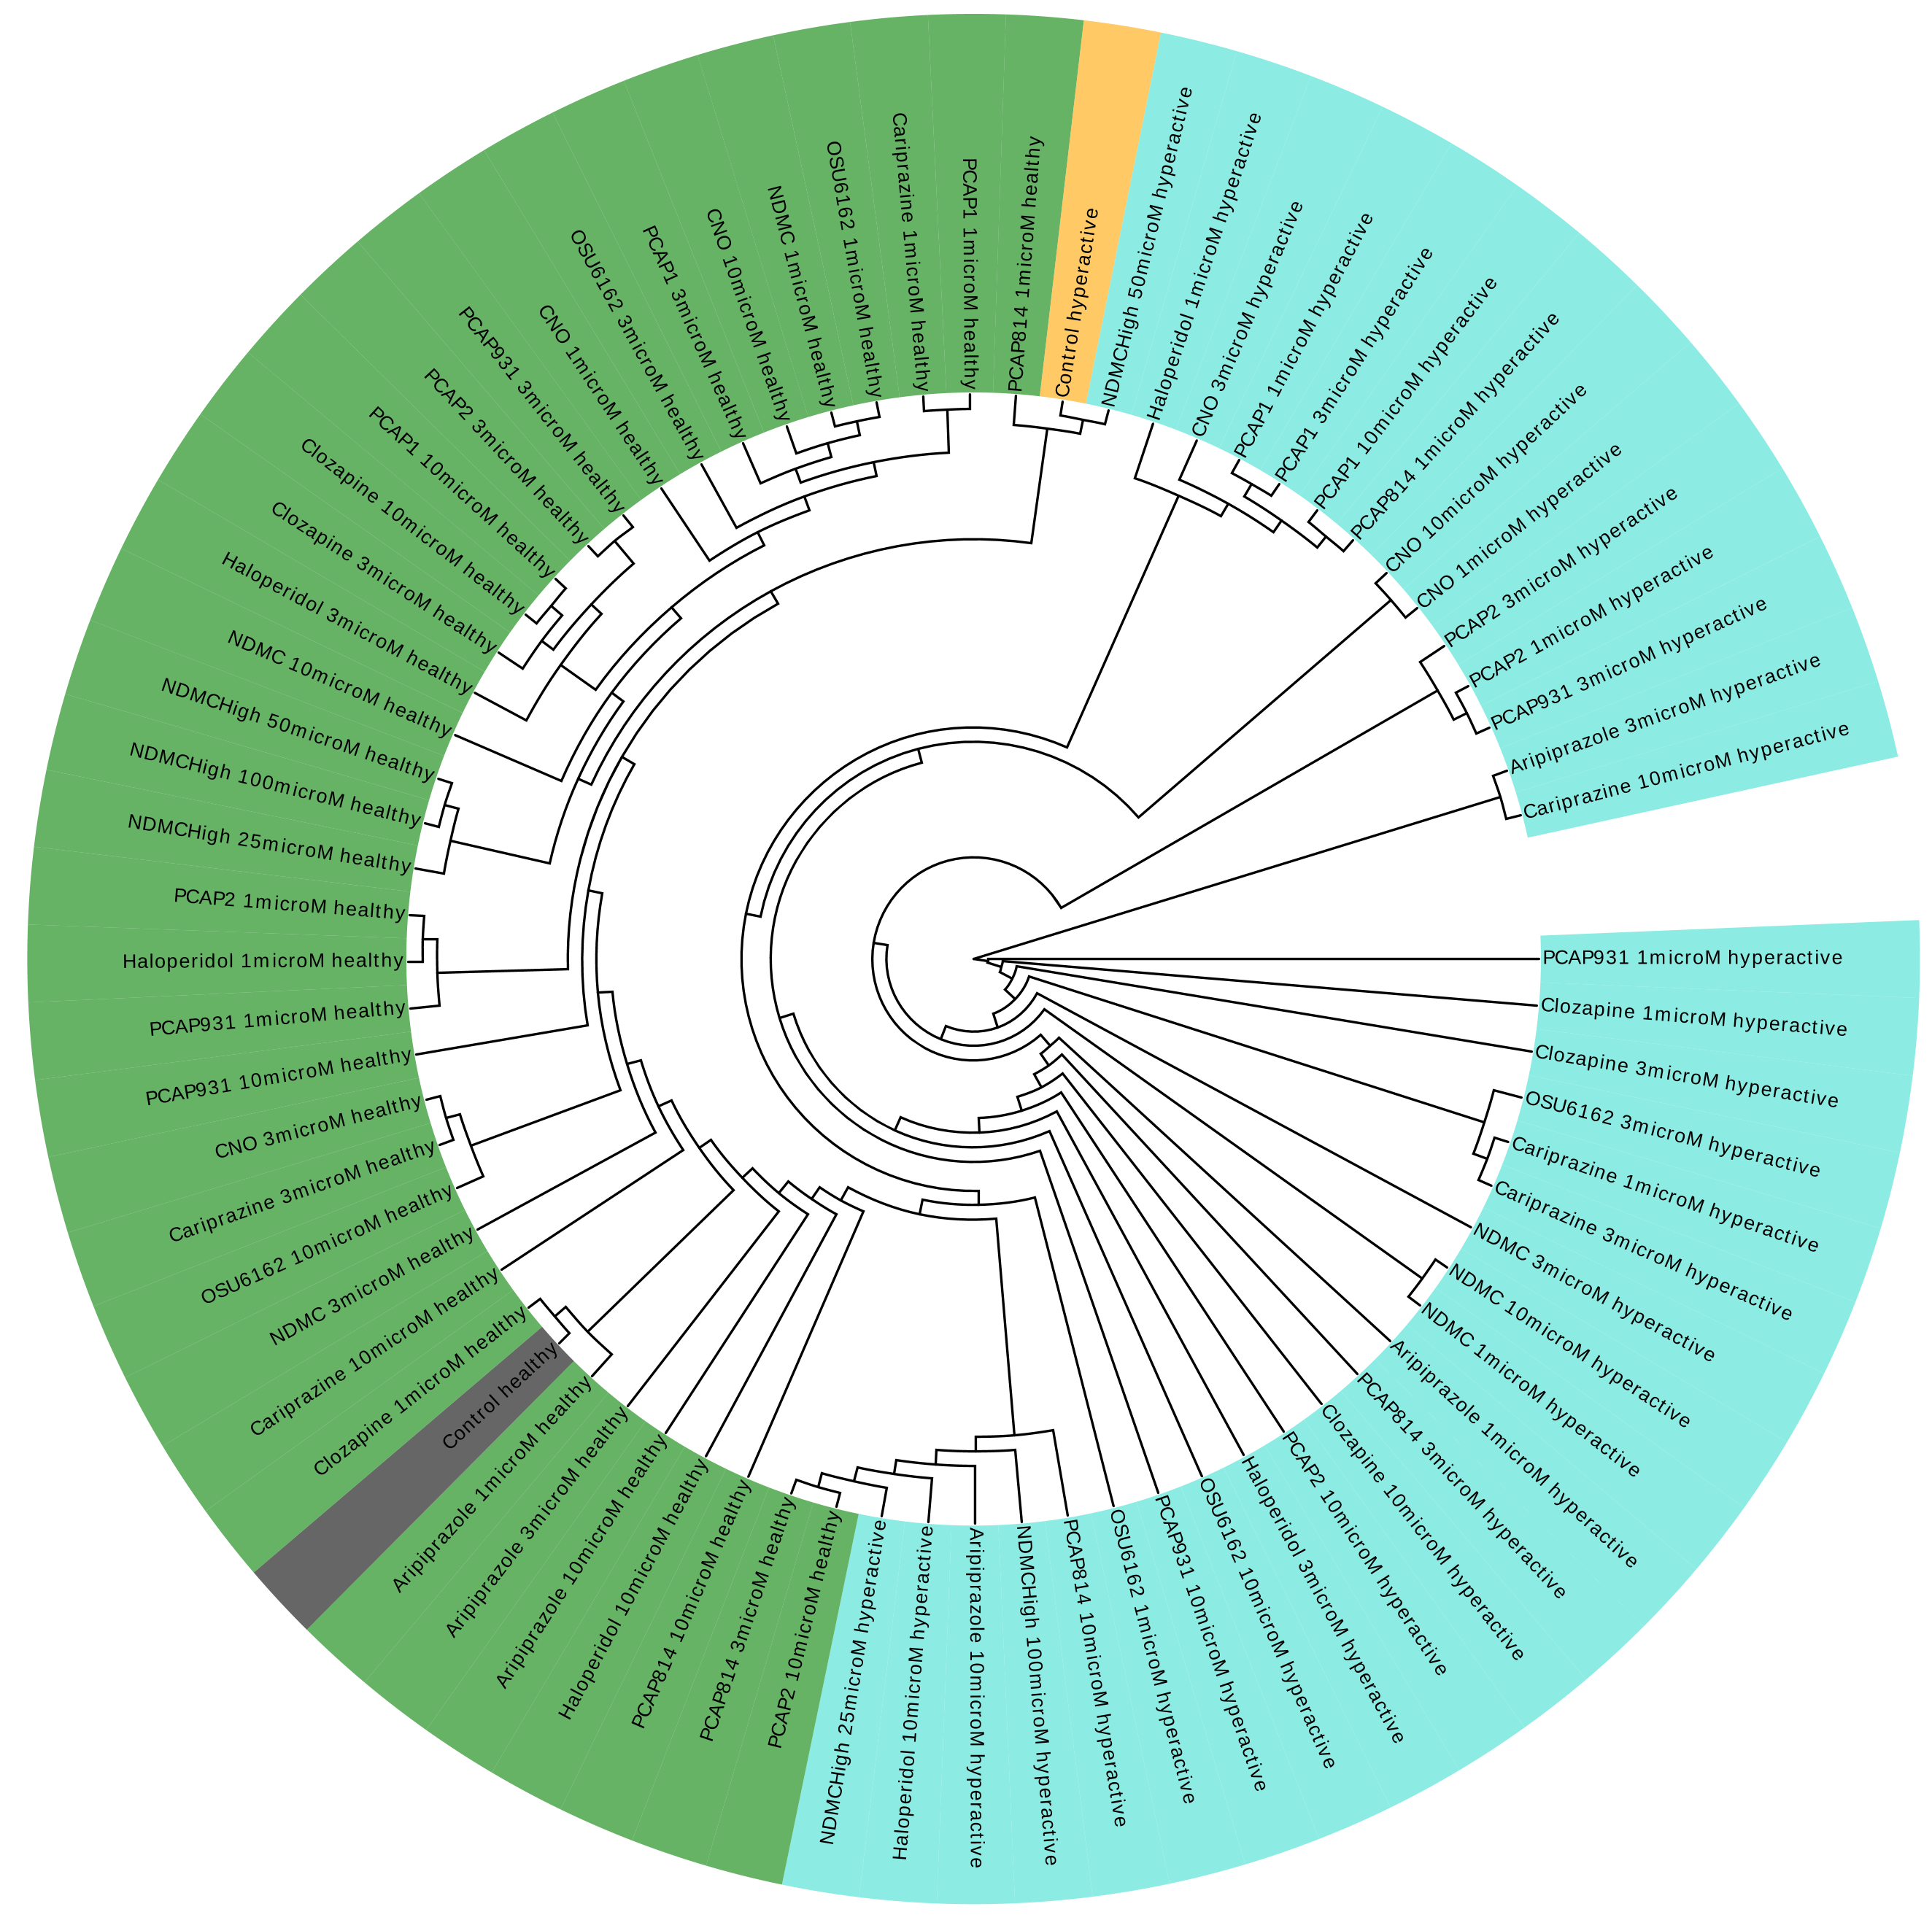
\includegraphics[width=8cm,height=7.5cm]{DarkApoHighB1.png}
\caption{Circular cladogram, representing Euclidean distances between the descriptive statistics of all experimental groups in the healthy and hyperactive condition, where the turn and turn transition descriptive statistics were obtained per bout length stratum.}
\end{center}
\end{figure}
\newpage
\begin{figure}[h!]
\begin{center}
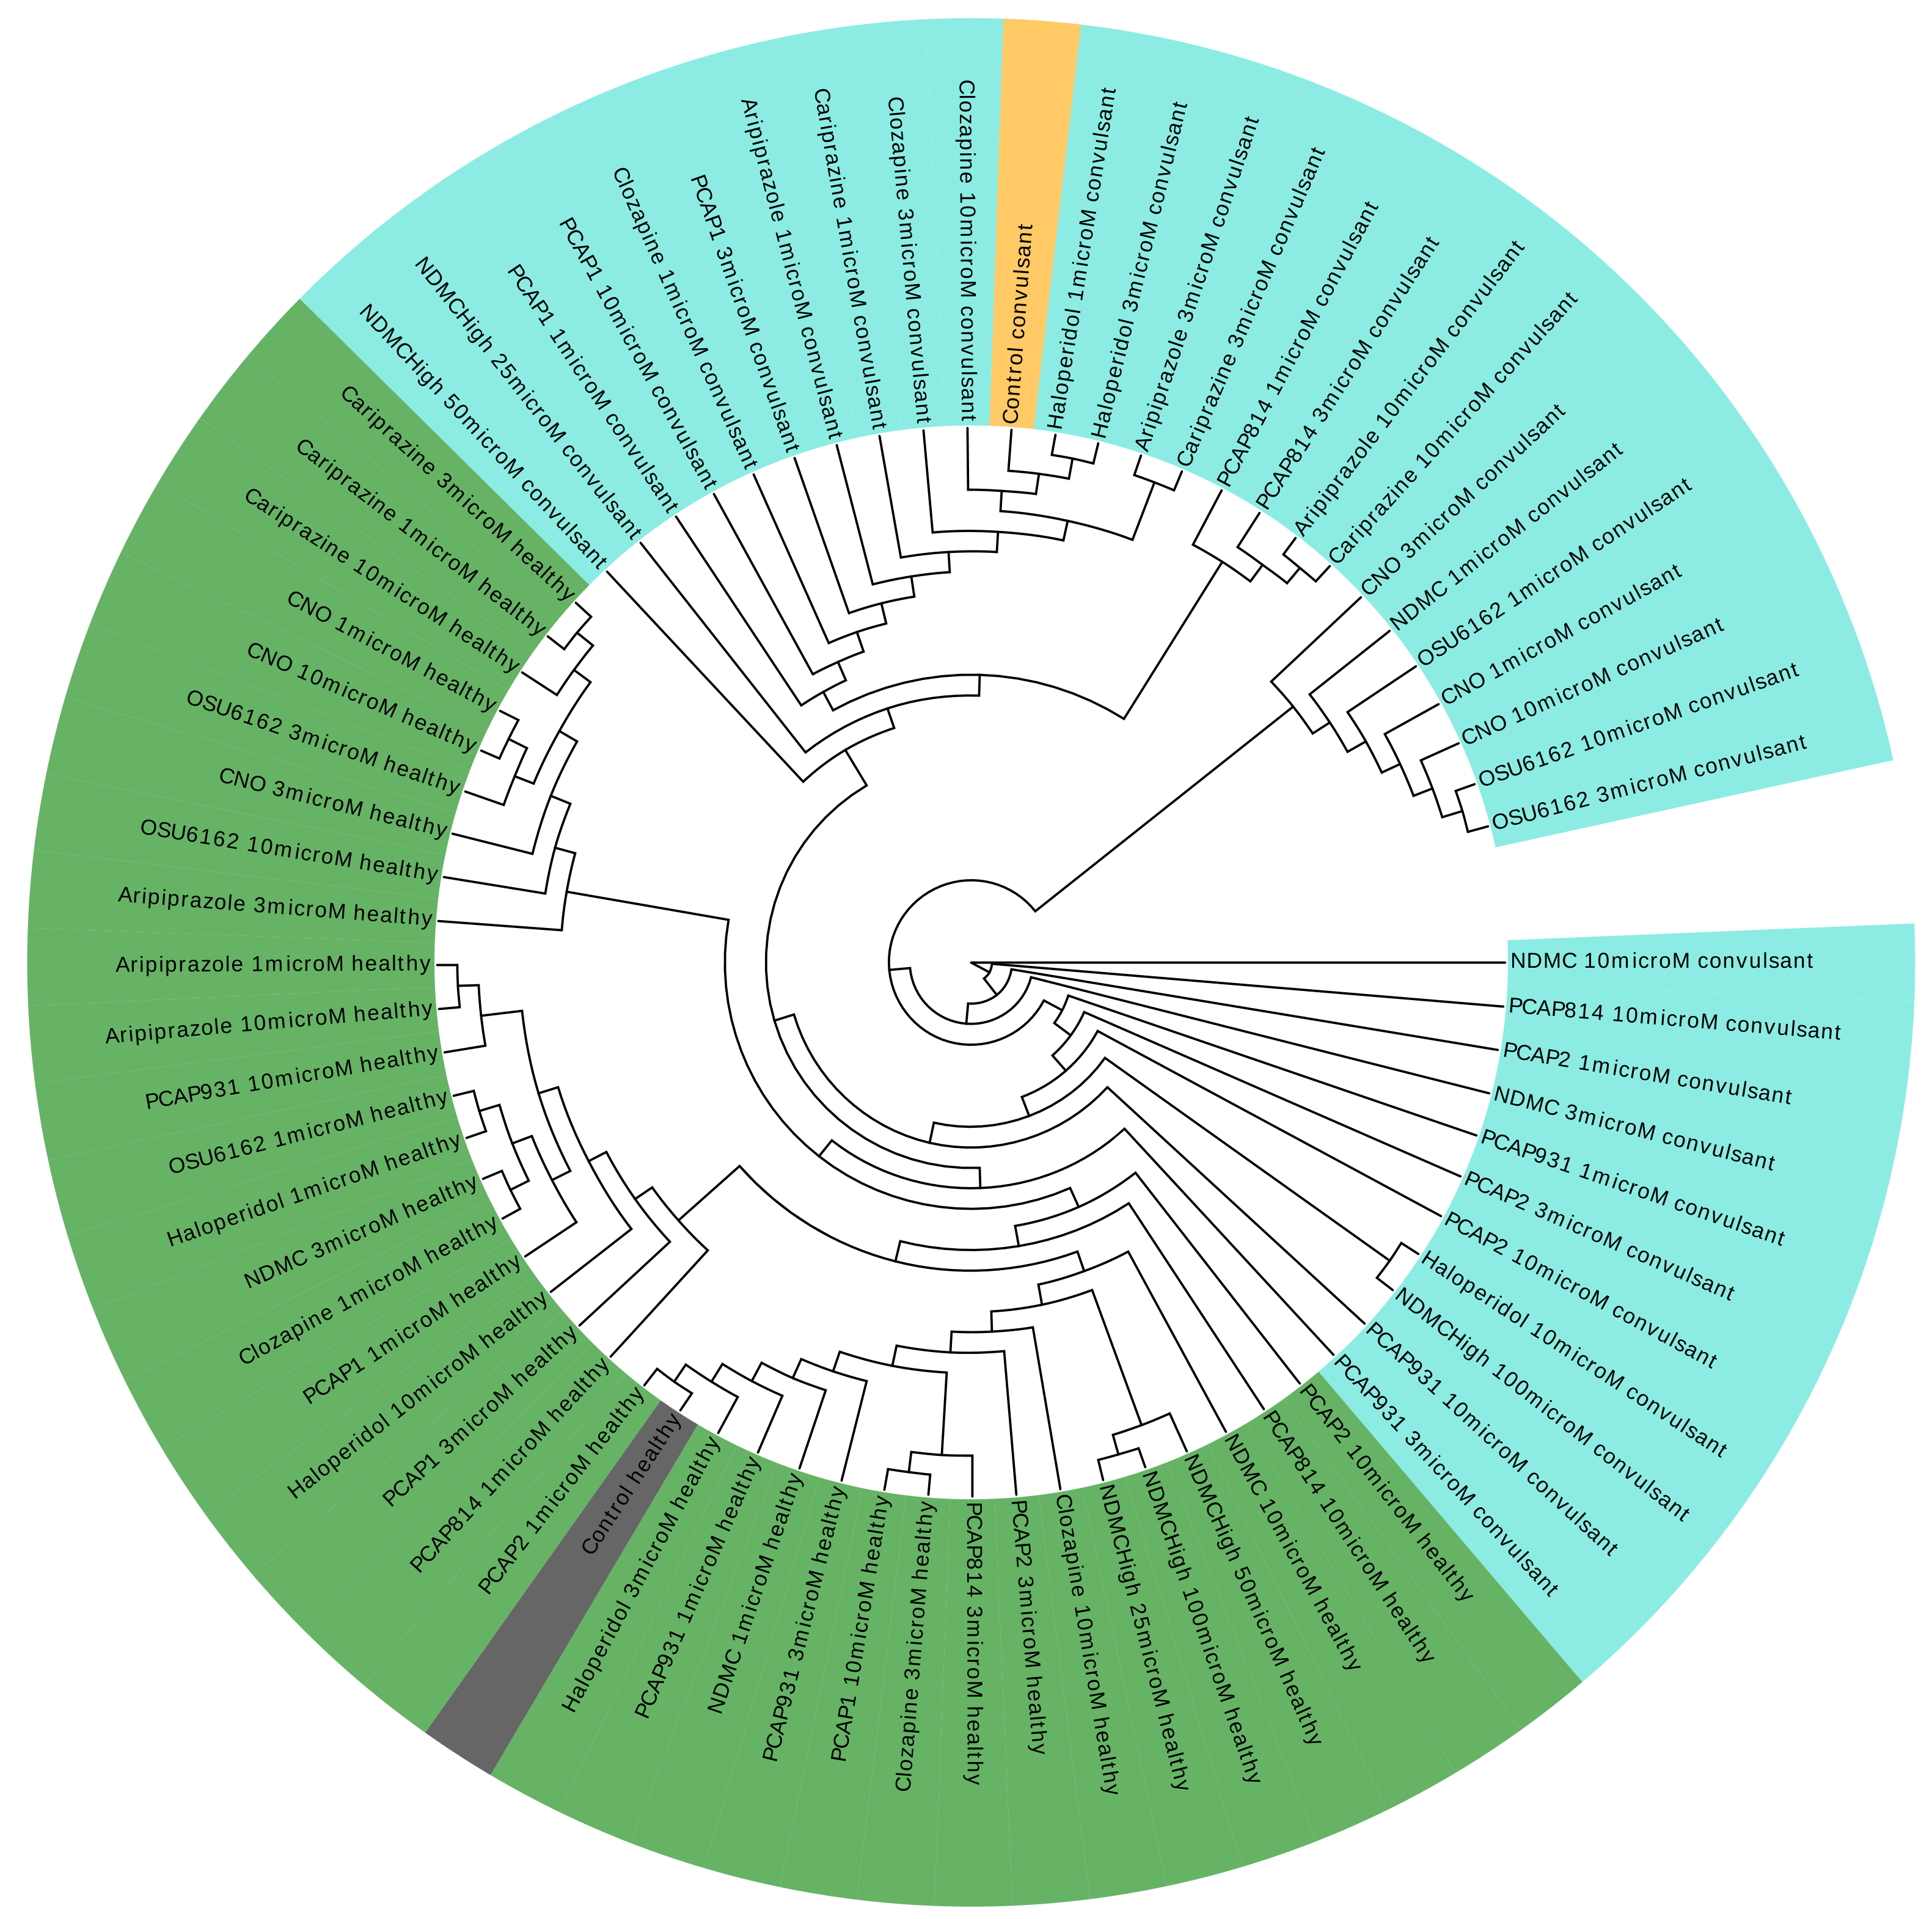
\includegraphics[width=8cm,height=7.5cm]{DarkPTZB2.png}
\caption{Circular cladogram, representing Euclidean distances between the descriptive statistics of all experimental groups in the healthy and convulsant condition, where the turn and turn transition descriptive statistics were not obtained per bout length stratum.}
\end{center}
\end{figure}
\begin{figure}[h!]
\begin{center}
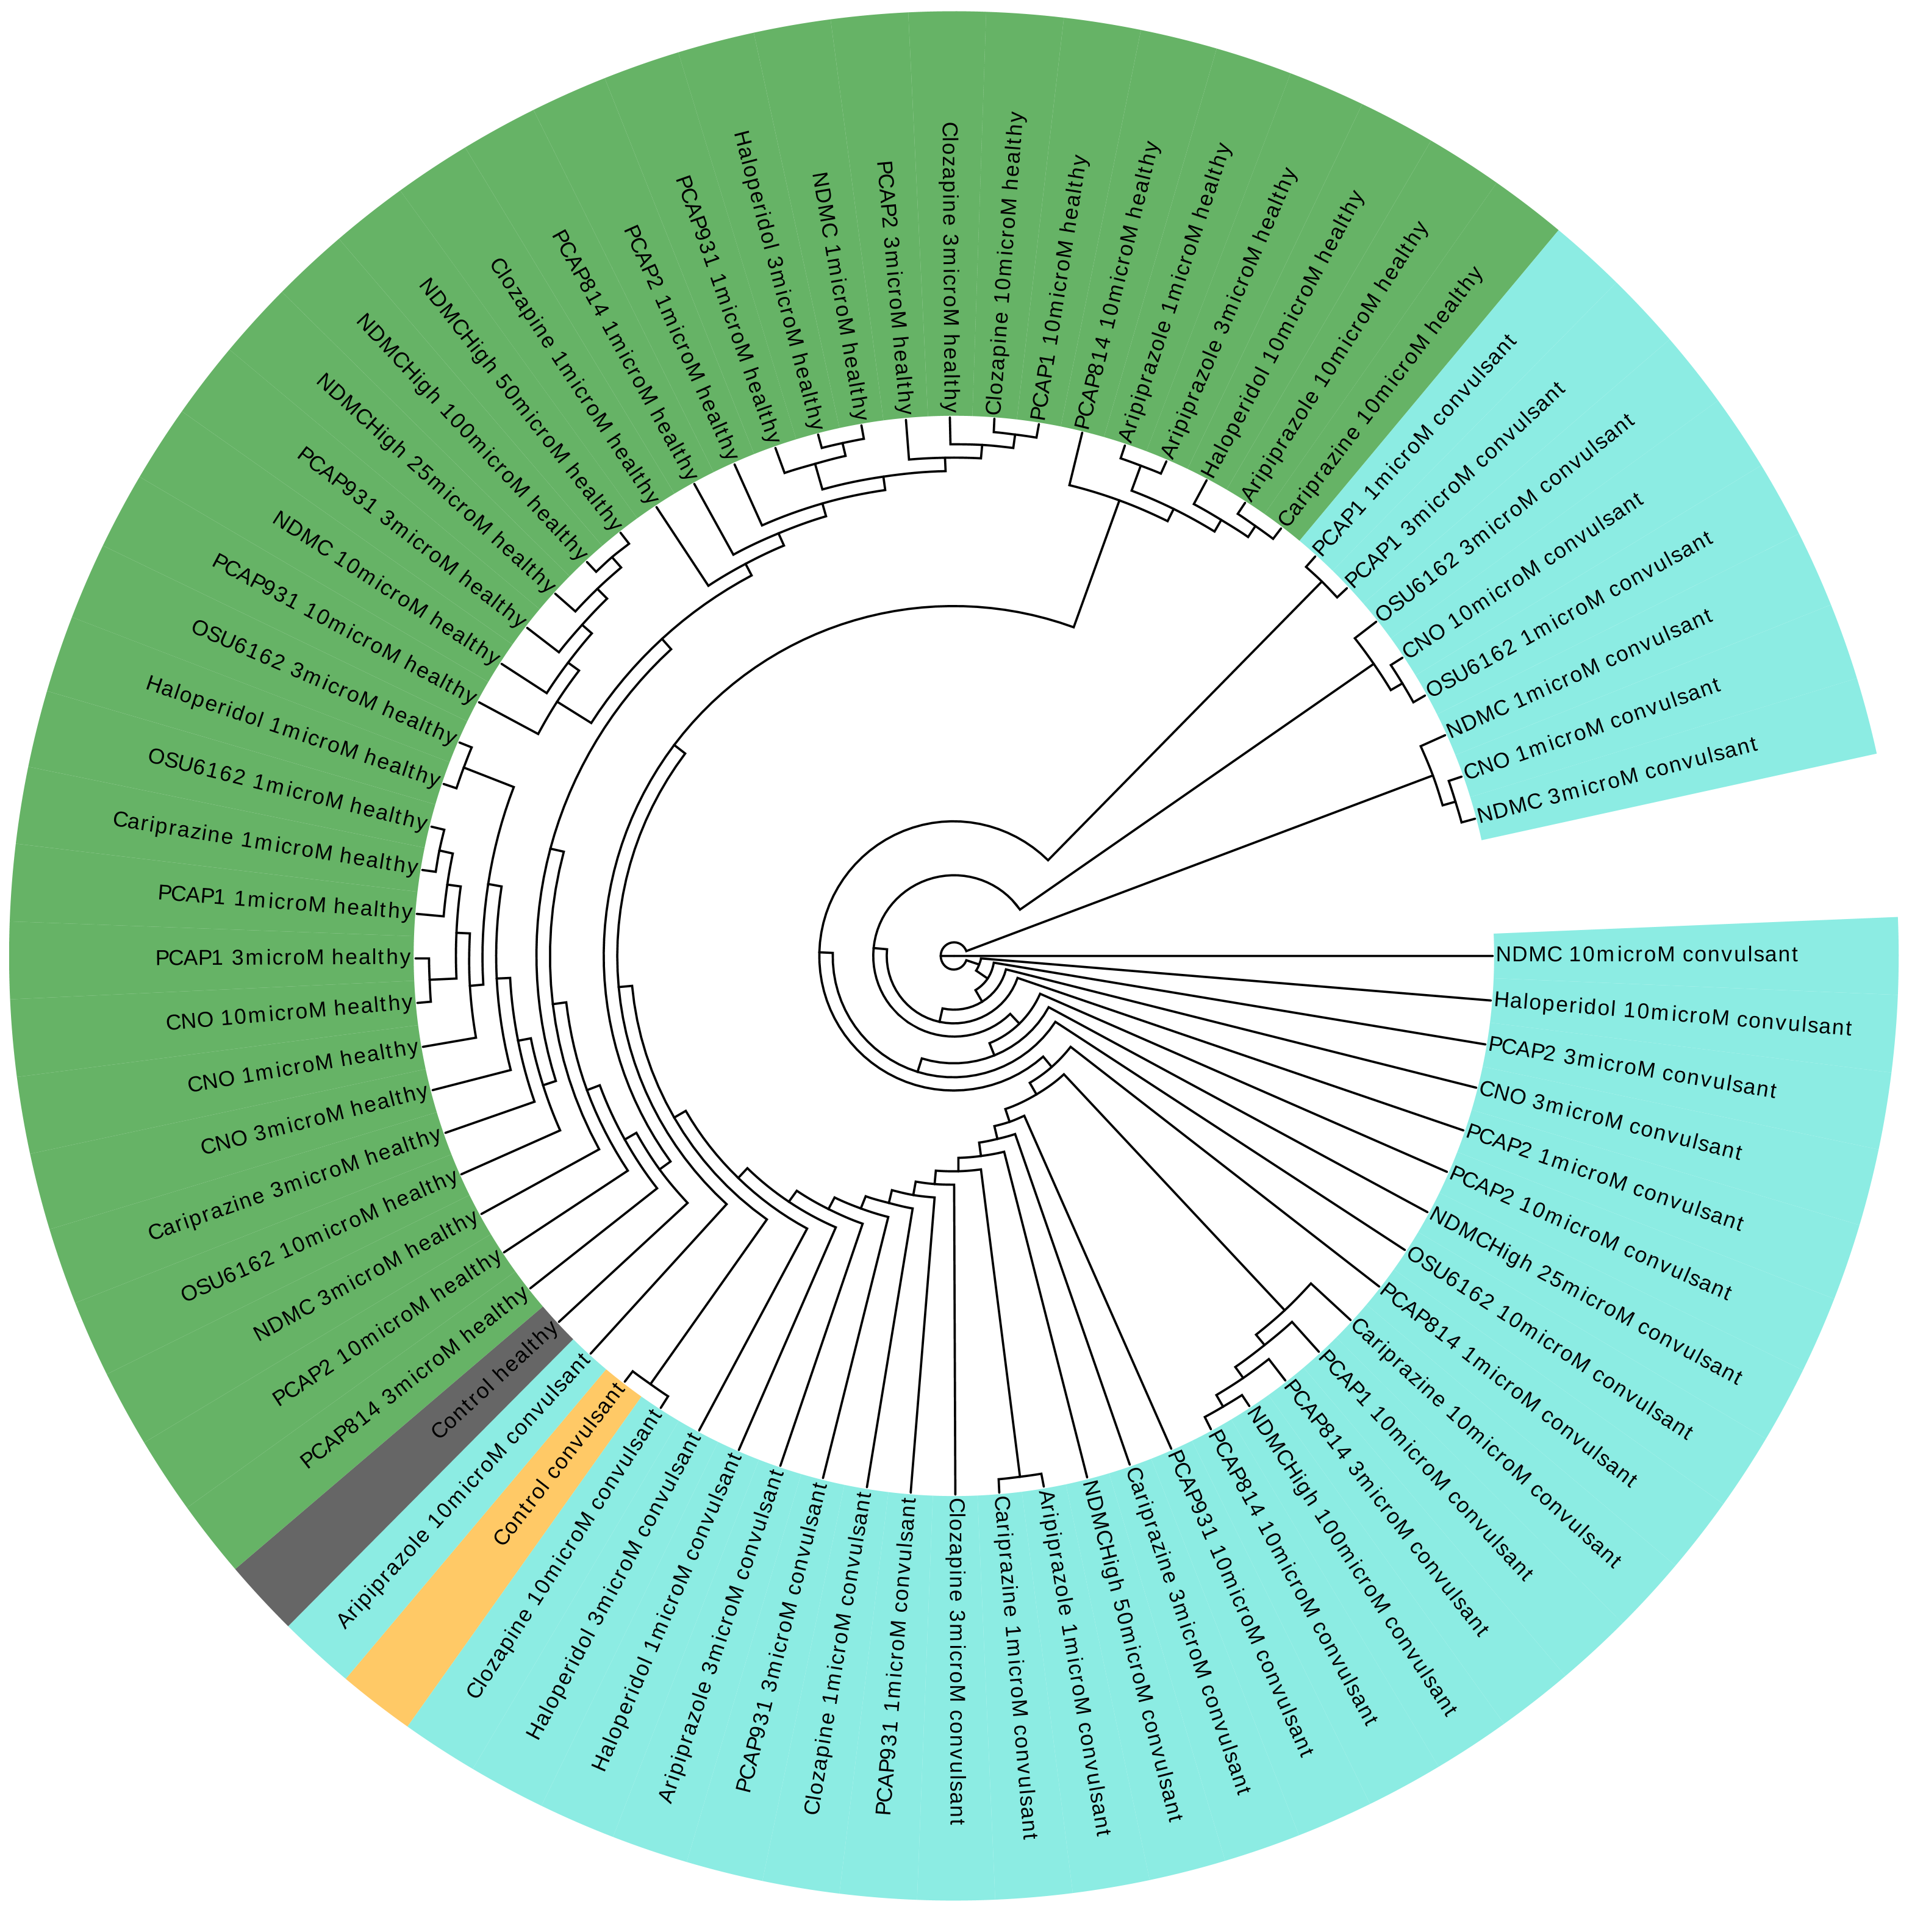
\includegraphics[width=8cm,height=7.5cm]{DarkPTZB1.png}
\caption{Circular cladogram, representing Euclidean distances between the descriptive statistics of all experimental groups in the healthy and convulsant condition, where the turn and turn transition descriptive statistics were obtained per bout length stratum.}
\end{center}
\end{figure}
\newpage
